\section{Projektplan}

\subsection{Projektstrukturplan}

\subsection{Meilensteinplan}
\subsubsection{Meilensteine}

\begin{itemize}
\item \textbf{M1} Ergebnis: Hardware ist beschafft, Schnittstellen sind definiert
\item \textbf{M2} Ergebnis: Ausleihstation funktionst�chtig
\item \textbf{M3} Ergebnis: Lotus Notes Schnittstelle funktioniert
\item \textbf{M4} Ergebnis: Hardware ist eingebaut und getestet
\item \textbf{M5} Ergebnis: Funktionierendes Ausleihsystem, Produkt ist abgenommen
\end{itemize}

\subsubsection{Arbeitspakete}

\begin{itemize}
\item \textbf{AP1} Hardware beschaffen (eine Woche)
\item \textbf{AP2} Hardware testen (eine Woche)
\item \textbf{AP3} Schnittstellenanalyse (eine Woche)
\item \textbf{AP4} Testaufbau Ausleihstation (eine Woche)
\item \textbf{AP5} Programmieren der Ausleihsoftware (vier Wochen)
\item \textbf{AP6} Abschlusstest der Software (eine Woche)
\item \textbf{AP7} Implementieren und Test der Lotus Notes Schnittstelle  (acht Wochen)
\item \textbf{AP8} Aufbau des Systems / Installation Software  (eine Woche)
\item \textbf{AP9} Abschlusstest des gesamten Systems (eine Woche)
\item \textbf{AP10} Einf�hrung, �bergabe und Abschlusstest (eine Woche)
\end{itemize}

\begin{figure}[h]
\begin{center}
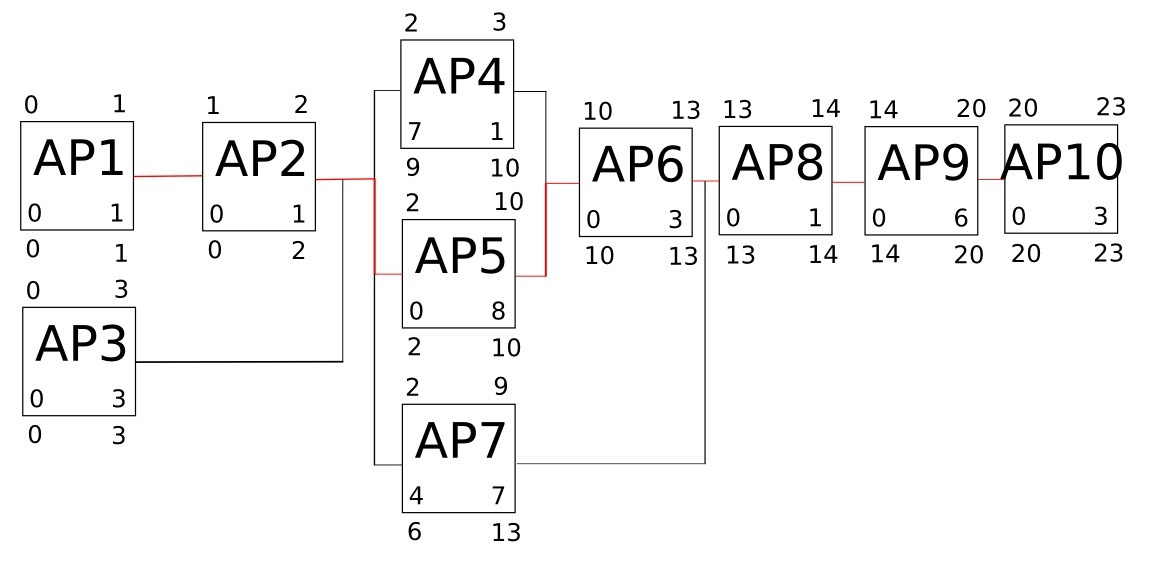
\includegraphics[width=0.8\textwidth]{abbildungen/netzplan.jpg}
\caption{Netzplan}
\end{center}
\end{figure}

\subsection{GANTT-Chart (Balkenplan)}
\begin{figure}[h]
\begin{center}
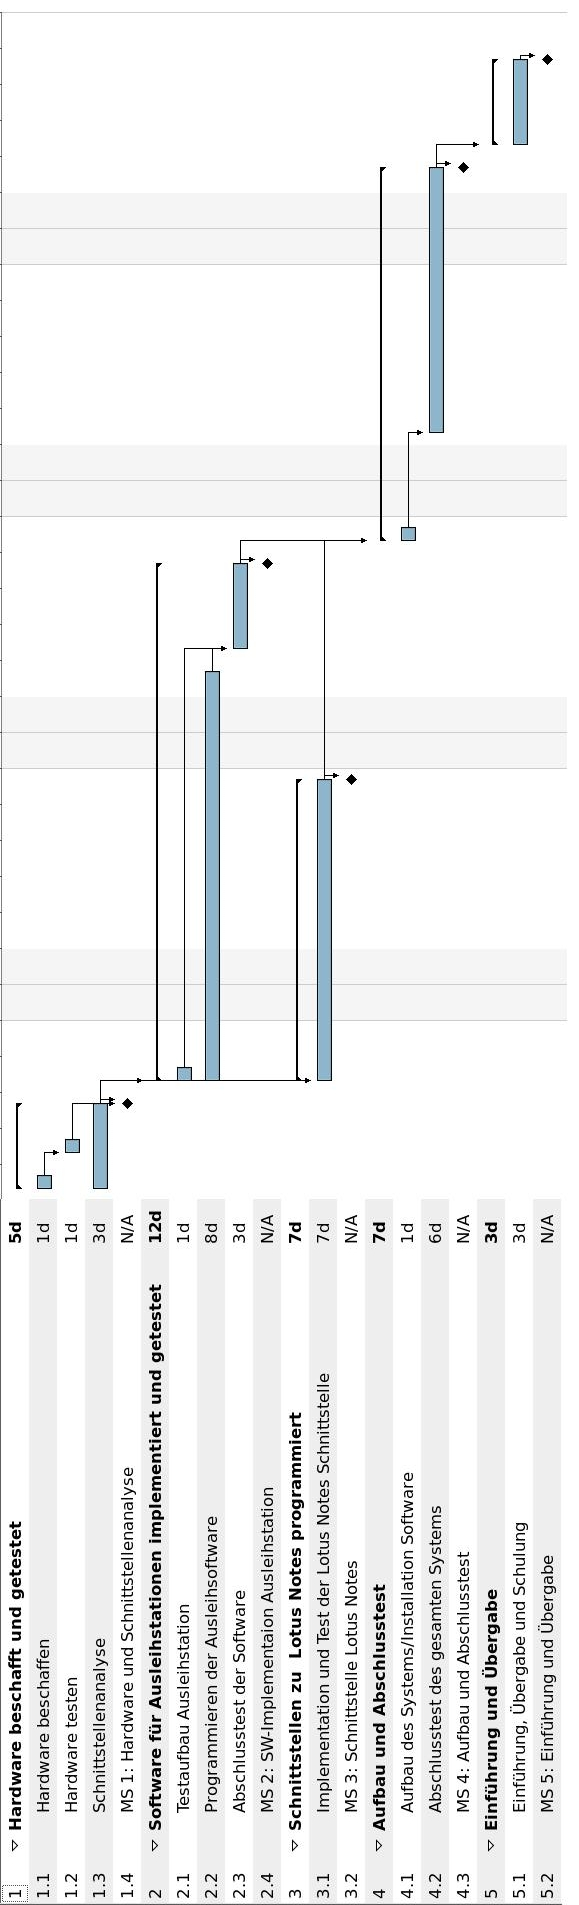
\includegraphics[width=0.4\textwidth] {abbildungen/gantt.jpg}
\caption{GANTT-Chart}
\end{center}
\end{figure}

\subsection{Kostens�tze}
Folgende Kostens�tze werden angenommen:
\begin{itemize}
\item 25 Euro f�r den einfachen Arbeiter
\item 35 Euro f�r den Denker
\end{itemize}

\subsection{Aufwands- und Kostensch�tzung}
\paragraph*{}
Die Kosten f�r die Hardware betragen laut Tabelle 5 703,62 Euro. Kosten von 8240 Euro f�r das Personal ergibt sich aus Tabelle 4. Somit entstehen Gesamtkosten von voraussichtlich 8943,62 Euro.

\begin{table}[h]
\caption{Aufwands- und Kostensch�tzung}
\begin{tabular}[h]{|p{0,6cm}|p{5cm}|p{4,3cm}|p{2cm}|p{2cm}|}
\hline
\textsc{Nr} & \textsc{Aktivit�t} & \textsc{Rollen} & \textsc{Aufwand} & \textsc{Kosten}\\
\hline
1.1 & Hardware beschafft & Hard- und Software & 1 Tag & 8 mal 25 Euro\\
1.2 & Hardware getestet & Hard- und Software & 1 Tag & 8 mal 25 Euro\\
1.3 & Schnittstellenanalyse & Hard- und Software & 3 Tage & 24 mal 35 Euro\\
2.1 & Testaufbau Ausleihstation & Hard- und Software & 1 Tag & 8 mal 25 Euro\\
2.2 & Programmieren der Ausleihsoftware & Hard- und Software & 8 Tage & 64 mal 35 Euro\\
2.3 & Abschlusstest der Software & Hard- und Software & 3 Tage & 24 mal 25 Euro\\
3.1 & Implementation und Test der Lotus Notes Schnittstelle & Ansprechpartner Lotus Notes & 7 Tage & 56 mal 35 Euro\\
4.1 & Aufbau des Systems/Installation Software & Hard- und Software & 1 Tag & 8 mal 25 Euro\\
4.2 & Abschlusstest des gesamten Systems & Auftraggeber & 6 Tage & 48 mal 25 Euro\\
5.1 & Einf�hrung, �bergabe und Schulung & Auftraggeber & 3 Tage & 24 mal 25 Euro\\
\hline
\end{tabular}
\end{table}

\begin{table}[h]
\caption{Hardware Kosten}
\rotatebox{90}{
\begin{tabular}[h]{|p{3cm}|p{3,5cm}|p{2,8cm}|p{2,8cm}|p{8cm}|}
\hline
\textsc{Beschreibung} & \textsc{Bezeichnung} & \textsc{St�ckpreis} & \textsc{Gesamtpreis} & \textsc{Link zum Hersteller}\\
\hline
Kamera & SAFESCAN 282W & 239.00 EUR & 239.00 EUR & \url{http://www.safescan.com/DE/productDetail/46/114/Safescan282W.html}\\
\hline
Barcodescanner & Metrologic 3580 Quantum USB schwarz & 297,02 EUR & 297,02 EUR &
\url{http://barcodescanner.rcf-shop-mall01.de/barcodescanner/metrologic_3580_quantum_usb_schwarz_von_,pd1050!0,,01056_MK3580-31A38.html}\\
\hline
T�rschloss & Kartenleser Kartenschloss Kemo M068 & 7,80 EUR & 7,80 EUR &
\url{http://www.luedeke-elektronic.de/products/Elektronik-Module/Sicherheit-Ueberwachung/Kartenleser-Kartenschloss-Kemo-M068.html}\\
\hline
Karten f�r T�rschloss & 20x5 Ersatzkarten f�r Kartenleser Kartenschloss Kemo M068 & 7,99 EUR & 159,80EUR & \url{http://www.luedeke-elektronic.de/products/Elektronik-Module/Sicherheit-Ueberwachung/Kartenleser-Kartenschloss-Kemo-M068.html}\\
\hline
\end{tabular}
}
\end{table}